\section{Congestion Control in a Diverse World}
%% Is coping too weak of a term?
\label{s:diversity}

In \S\ref{s:tcpaware}, we discussed the costs and benefits of
TCP-awareness. Here we report on further investigations to understand
the differing performance of TCP-naive and TCP-aware Tao protocols by
inspecting their transmissions in the time domain, when contending
with TCP cross-traffic (Figure~\ref{fig:explain}). The results show
that TCP-awareness is a complicated phenomenon, which yields higher
delays in isolation but smaller delays when contending with TCP. It is
not simply a question of ``more aggressive'' or ``less aggressive''
congestion-control.

\begin{figure*}
\centering
\begin{subfigure}[b]{0.4\textwidth}
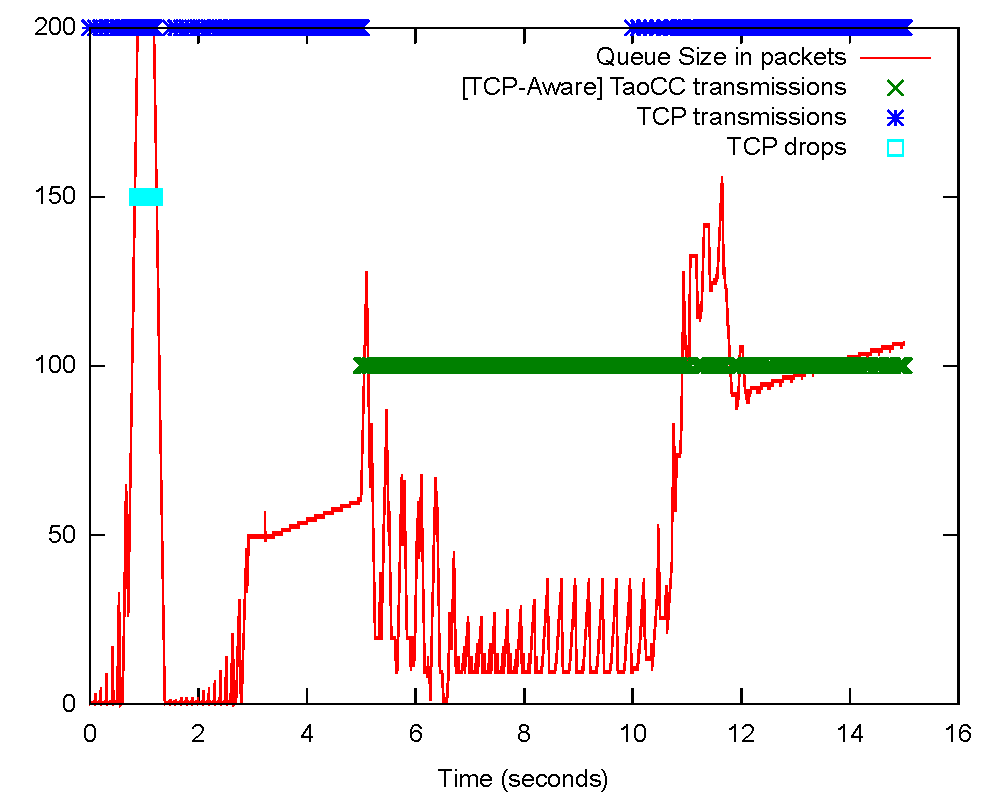
\includegraphics[width=\textwidth]{tx-queue-aware.pdf}
\end{subfigure}
\begin{subfigure}[b]{0.4\textwidth}
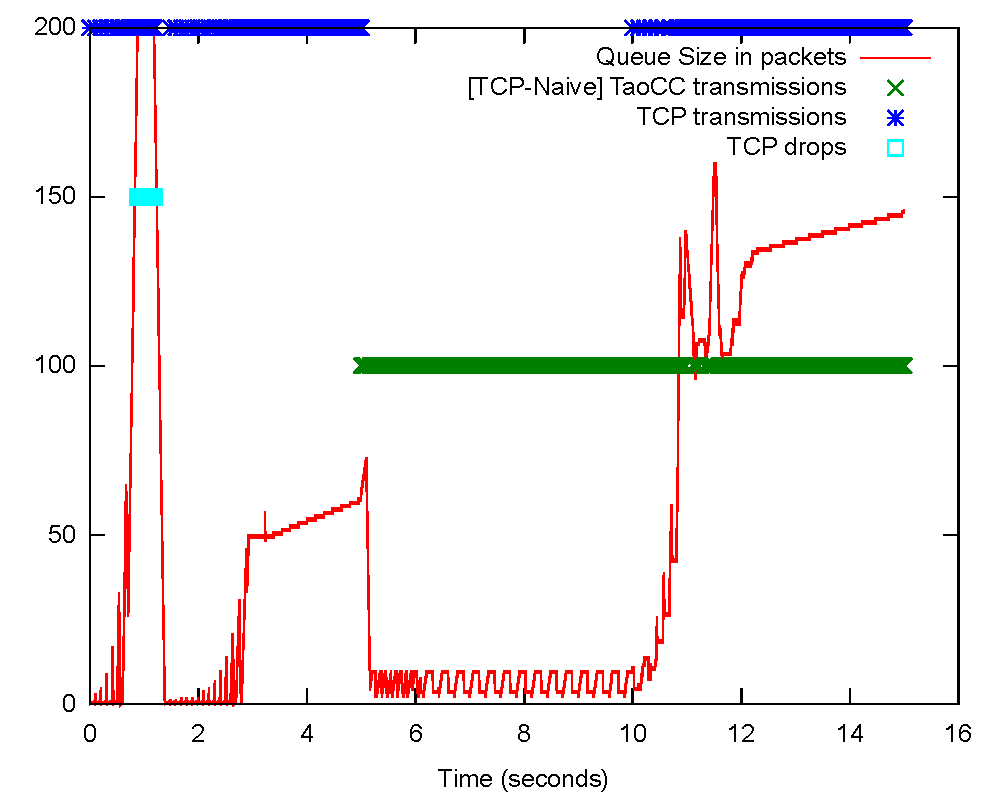
\includegraphics[width=\textwidth]{tx-queue-naive.pdf}
\end{subfigure}
\caption{In isolation, a TCP-aware Tao protocol is more aggressive than it needs to be, leading to higher delays. But when competing with TCP cross-traffic, the Tao protocol achieves the reverse situation---lower queueing delay, and higher throughput, than the TCP-naive Tao protocol.}
\label{fig:explain}
\end{figure*}


\label{ss:backward}

\subsection{The price of sender diversity}
\label{ss:forward}

\begin{figure}
\centering
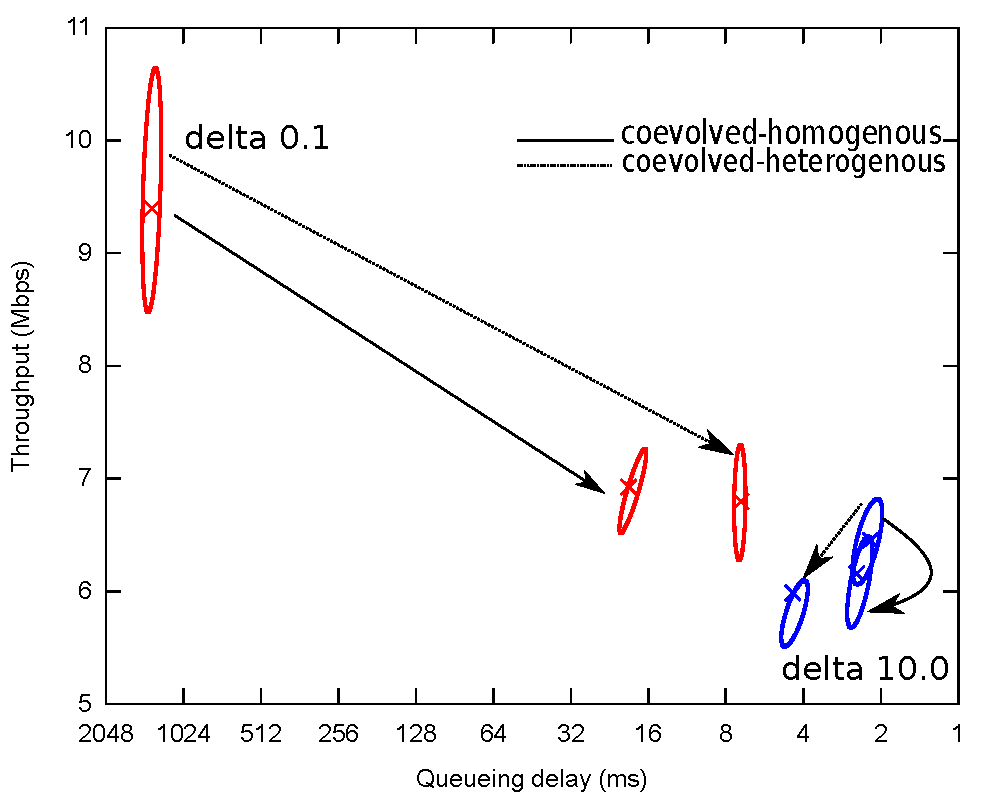
\includegraphics[width=\columnwidth]{diversity-both.pdf}
\caption{Co-designing Tao protocols for differing objectives brings both protocols towards a middle ground, but preserves some room for diversity.}
\label{fig:diversity-training}
\end{figure}

We further generalize the notion of TCP-awareness by asking whether it
is possible to design multiple new congestion-control protocols to
simultaneously achieve differing objection's when contending on the
same bottleneck link.

We investigate the possibility of co-developing congestion-control protocol
for differing sender objectives. We consider two extreme cases: a sender
that weighs throughput ten times over delay ($\delta=0.1$), and a sender that
weighs delay ten times over throughput ($\delta=10.0$).

We suspected that achieving diversity in this manner may not be
possible, reasoning that endpoints that share the same bottleneck link
will necessarily experience the same queueing delay, and therefore
endpoints that achieve an optimal throughput-to-delay tradeoff will
experience the same overall performance.

But contrary to this hypothesis, our findings are that it is possible
to co-develop congestion control algorithms such that they can both
co-exist with each other and yet---because of variable duty
cycles---achieve some diversity in their chosen objectives.  Even when
running together, the delay-preferring sender sees lower delay than
the throughput-preferring sender, while the opposite is true with
throughput. When congestion-control protocols are co-developed, but
each sender runs homogeneously, each sender receives higher throughput
or lower delay, as the case they may be.

However, coexistence does come at a price to the throughput-preferring
sender, which suffers a loss in throughput by being ``nice" to the
delay-preferring sender. By comparison, the performance of the
delay-preferring sender is affected only modestly.
